\documentclass[11pt]{article}
\usepackage{amsmath}
\usepackage{graphicx}
\usepackage{amsthm}
\usepackage{algpseudocode}
\usepackage{placeins}
\begin{document}
\title{Assignment 1 - B553}
\author{Chaitanya Bilgikar (cbilgika)\\
		Debpriya Seal (debseal)}
\maketitle
\section*{Question 1}
Total number of ways of arranging 4 parakeets = 8!\\
Total number of arrangements in which no two adjacent parakeets have the same color = 2!(4!*4!)\\
\begin{equation*}
\begin{split}
\text{Pr(No two adjacent parakeets have the same color)} &= \frac{2!(4!*4!)}{8!}\\
&=\frac{1}{35}\\
&=0.02857142857143
\end{split}
\end{equation*}
\section*{Question 2}
\subsection*{(a)}
For a CPU to have all functioning cores, means that all cores should not be defective. Since the defects in the cores are all independent of one another,
\begin{equation*}
\begin{split}
\text{Pr(no core has defect)} & = (0.7)^8\\
&=0.05764801
\end{split}
\end{equation*}
\subsection*{(b)}
First we calculate the probability of each type of computer being made. We can consider this as a binomial distribution with 8 trials and the probability of success $p$ as $0.7$. The binomial probability can be expressed as:
\begin{equation*}
B(8,0.7,x) = \binom{8}{x}*(0.7)^x * (0.3)^{(8-x)}
\end{equation*}
\begin{equation*}
\begin{split}
\text{Pr(Great model)} &= \text{Pr(one,two or three cores working)}\\
&=\sum_{x=1}^3\left(\binom{8}{x}*(0.7)^x * (0.3)^{8-x}\right)\\
&=0.05790\\ \\
\text{Pr(Advanced model)} &= \text{Pr(at least 4 cores functioning)}\\
&=\sum_{x=4}^7\left(\binom{8}{x}*(0.7)^x * (0.3)^{8-x}\right)\\
&= 0.88438\\ \\
\text{Pr(Extreme model)} &= \text{Pr(all 8 cores functioning)}\\
&= (0.7)^8\\
&=0.05764801
\end{split}
\end{equation*}
Expectation of number of each of these models is then given by the equation:
\begin{equation*}
E(X) = \sum_{x\in X} \left(x*pr(x)\right)
\end{equation*}
Using this, we get,
\begin{equation*}
\begin{split}
E(\text{Great model}) &= 1000*0.05790\\
&=57.9 \approx 58\\ \\
E(\text{Advanced model}) &= 1000*0.88438\\
&=884.38 \approx 884\\ \\
E(\text{Extreme model}) &= 1000*0.05764801\\
&=57.64801 \approx 58
\end{split}
\end{equation*}
\subsection*{(c)}
Expected revenue can be calculated as:
\begin{equation*}
\begin{split}
E(revenue) &= \$(58*50*0.057) +\$(100*884*0.884) + \$(58*1000*.057)\\
&=\$81,616
\end{split}
\end{equation*}
\section*{Question 3}
Let us define the following events:
\begin{equation*}
\begin{split}
A_1 &= \text{Judge 1 votes guilty}\\
A_2 &= \text{Judge 2 votes guilty}\\
A_3 &= \text{Judge 3 votes guilty}\\
G &= \text{The person is guilty}
\end{split}
\end{equation*}
We are given the following things:
\begin{equation*}
\begin{split}
Pr(G) &= 0.7\\
Pr(A_1|G) &= Pr(A_2|G) = Pr(A_3|G) = 0.7\\
Pr(A_1|\bar{G}) &= Pr(A_2|\bar{G}) = Pr(A_3|\bar{G}) = 0.2
\end{split}
\end{equation*}
\subsection*{(a)}
Using Bayes rule,
\begin{equation*}
\begin{split}
Pr(G|A_1) &= \frac{Pr(A_1|G)*Pr(G)}{Pr(A_1)}\\
&=\frac{Pr(A_1|G)*Pr(G)}{\left(Pr(A_1|G)*Pr(G)\right) + \left(Pr(A_1|\bar{G})*Pr(\bar{G})\right)}\\
&=\frac{0.7*0.7}{\left(0.7*0.7\right)+\left(0.2*0.3\right)}\\
&=0.8909
\end{split}
\end{equation*}
\subsection*{(b)}
\begin{equation*}
\begin{split}
Pr(G|A_1,A_2,A_3) &= \left(\frac{Pr(G,A_1,A_2,A_3)}{Pr(A_1,A_2,A_3)}\right)\\
&=\left(\frac{Pr(A_1|G)*Pr(A_2|G)*Pr(A_3|G)*Pr(G)}{(\sum_{g\in G}Pr(A_1|G=g)*Pr(A_2|G=g)*Pr(A_3|G=g)*Pr(G=g))}\right)\\
&=\left(\frac{0.7^4}{(0.7^4)+(0.2^3*0.3)}\right)\\
&=0.9901
\end{split}
\end{equation*}
\subsection*{(c)}
\begin{equation*}
\begin{split}
Pr(A_3|\bar{A_1},\bar{A_2}) &=\frac{Pr(\bar{A_1},\bar{A_2},A_3)}{Pr(\bar{A_1},\bar{A_2})}\\
&= \frac{\Sigma_{g\in G} \left(Pr(\bar{A_1}|g)*Pr(\bar{A_2}|g)*Pr(A_3|g)*Pr(g)\right)}{\Sigma_{g\in G}\left(Pr(\bar{A_1}|g)*Pr(\bar{A_2}|g)*Pr(g)\right)}\\
&= \frac{0.0825}{0.255}\\
&= 0.3235
\end{split}
\end{equation*}
\section*{Question 4}
Consider a set of $k+1$ events of which $k$ are undesirable. Assume that the probability of the desired event is $p$. Then the expected number of trials to get the desired event is $\frac{1}{p}$ \cite{trial}.
\subsection*{(a)}
Since we have 3 of the 4 figurines, getting them in the next trial is an undesired event. Here the probability of getting the figurine that we want is $\frac{1}{4}$. Hence,
\begin{equation*}
E[\text{Number of trials to get one figurine}] = \frac{1}{p} = \frac{1}{\frac{1}{4}} = 4
\end{equation*}
\subsection*{(b)}
We can break down this question into four parts.
\begin{equation*}
\begin{split}
Pr(\text{Getting 1st new figurine}) &= 1\\
Pr(\text{Getting 2nd new figurine}) &= \frac{3}{4}\\
Pr(\text{Getting 3rd new figurine}) &= \frac{1}{2}\\
Pr(\text{Getting 4th new figurine}) &= \frac{1}{4}
\end{split}
\end{equation*}
Hence,
\begin{equation*}
\begin{split}
E[\text{Number of trials to get all four figurines}] &= 1 + \frac{1}{\frac{3}{4}} + \frac{1}{\frac{1}{2}} + \frac{1}{\frac{1}{4}}\\
&= 1 + \frac{4}{3} + 2 + 4\\
&=8.333
\end{split}
\end{equation*}
\section*{Question 5}
\begin{figure}[h]
\centering
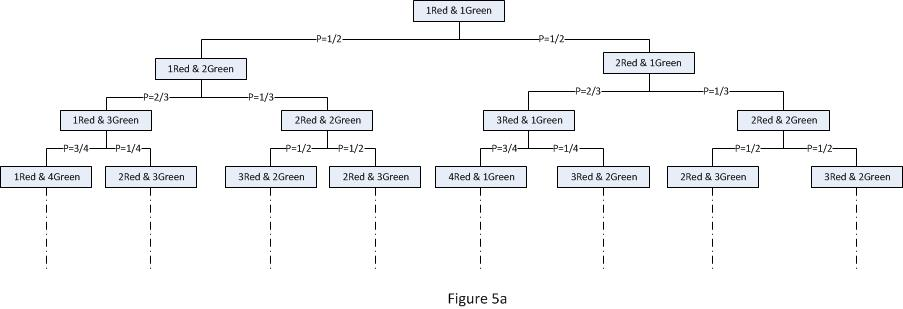
\includegraphics[scale=0.55]{Question5a_Figure1.jpg}
\caption{Graph for 5a}
\label{fig:fig1}
\end{figure}
\emph{Figure}~\ref{fig:fig1} demonstrates the graph can be generated for the given experiment. From it we get,
\begin{equation*}
Pr[R=1,G=(n+1)] = \left(\frac{1}{2}*\frac{2}{3}*\frac{3}{4}*\dotsm *\frac{n}{(n+1)}\right)
\end{equation*}
If we move down each path in the given graph we find the following:
\begin{equation*}
\begin{split}
Pr[R=1,G=(n+1)] &= \frac{1}{n+1}\\
Pr[R=2,G=n] &= \frac{1}{n+1}\\
Pr[R=n,G=2] &=\frac{1}{n+1}\\
Pr[R=n+1,G=1] &= \frac{1}{n+1}\\
&\text{where R,G are the number of red and green bills}
\end{split}
\end{equation*}
This shows that the probability of getting red bills and green bills is the same.
\subsection*{(a)}
By linearity of expectation, 
\begin{equation*}
\begin{split}
E[G-R] &= E[G] - E[R]\\
\text{From the observation above, we get,}\\
E[G-R]&=0
\end{split}
\end{equation*}
For the variance, we have the expression,
\begin{equation*}
\begin{split}
V[G-R] &= \sum_{-n}^n (x-\mu)^2*Pr(x)\\
\end{split}
\end{equation*}
Values of $G-R$ range from $-n$ to $n$\\
This can be split as:
\begin{equation*}
\begin{split}
V[G-R] &= \sum_{-n}^0\left((x-\mu)^2*Pr(x)\right) + \sum_{1}^n \left((x-\mu)^2*Pr(x)\right)
\end{split}
\end{equation*}
Since our $\mu$ is 0, we get
\begin{equation*}
\begin{split}
V[G-R] &= 2*\sum_{1}^n (x)^2*Pr(x)\\
\text{Substituting the values from above, we get,}\\
&=2* 44469.1666\\
&=88938.33
\end{split}
\end{equation*}
\subsection*{(b)}
If we need to owe the government at least \$300, then,
\begin{equation*}
\begin{split}
R-G &\geq 300 \\
\text{and}\\
R + G &= 367\\
\Rightarrow G & \geq 334\\
&= \sum_{x=334}^{365}\left(x^2*Pr(x)\right)\\
&= 31.55 \quad \text{\emph{(by calculation)}}
\end{split}
\end{equation*}
Parts (a) and (b) have been discussed with \cite{moiz}
\subsection*{(c)}
\begin{figure}[h]
\centering
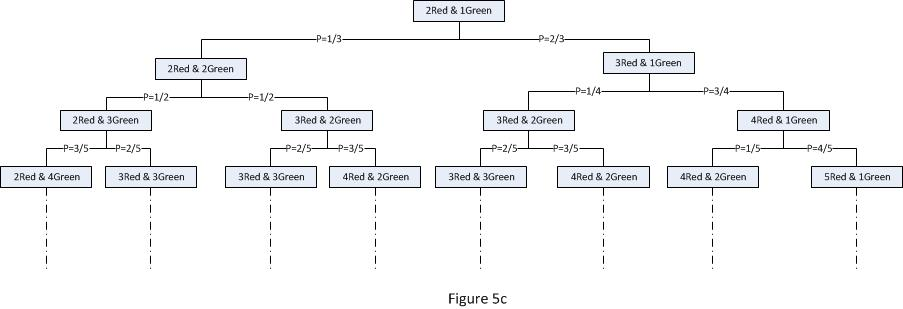
\includegraphics[scale=0.55]{Question5c_Figure1.jpg}
\caption{Graph for 5c}
\label{fig:fig2}
\end{figure}

In this case \emph{Figure}~\ref{fig:fig2} shows the graph. As in part (a) of this question we get,
\begin{equation*}
\begin{split}
Pr[R=2,G=(n+1)] &= \left(\frac{1}{3}*\frac{2}{4}*\frac{3}{5}*\dotsm *\frac{(n-1)}{(n+1)}\right)\\
&=\frac{2}{n*(n+1)}\\
Pr[R=n+2,G=1] &= \left(\frac{2}{3}*\frac{3}{4}*\frac{4}{5}*\dotsm *\frac{n}{(n+1)}\right)\\
&=\frac{2}{(n+1)}
\end{split}
\end{equation*}
To get the expectation, we again use linearity of expectation, after which we get,
\begin{equation*}
\begin{split}
E[G-R] &= E[G] - E[R]\\
&=\sum_1^{n+1}\left(x*Pr(x)\right) - \sum_1^{n+2}\left(x*Pr(x)\right)\\
&=\sum_1^{n+1}\left(x*\frac{2}{(n-x)(n+1)}\right) - \sum_1^{n+2}\left(x*\frac{2}{(n-x)(n+1)}\right)\\
&=-\frac{(n+2)}{(n+1)}\\
&=-\frac{367}{366}\\
&=-1.027
\end{split}
\end{equation*}
Another way to solve this would be to consider the use of graph theory.
Notice that the graph is a binary tree of depth 365. Hence the number of nodes is $2^{365}$. Also note that at depth $k$, there are $k-1$ nodes that are repeated $k$ times (that is, there are $k-1$ nodes that have the same combination of green bills and red bills as each other, and there are $k$ such nodes).So, at level 365, we will have 364 nodes that have the same combination of green and red bills and there are 365 such nodes. So, the probability of $r$ red bills and $g$ green bills can be computed by using a modification of Djikstra's algorithm (where the path length is a multiplication of the individual edges, each edge representing the probability of picking a new bill) to these nodes.  
\begin{thebibliography}{10}
\bibitem{trial}Mathematical expectation from CodeChef \emph{http://www.codechef.com/wiki/tutorial-expectation}
\bibitem{moiz}Nasheed Moiz, Shrutika Poyrekar
\end{thebibliography}
\end{document}
